% !TeX spellcheck = en_GB
% This is LLNCS.DOC the documentation file of
% the LaTeX2e class from Springer-Verlag
% for Lecture Notes in Computer Science, version 2.4
\documentclass{llncs}
\usepackage{llncsdoc}
\usepackage{graphicx} 
\usepackage{booktabs}
\usepackage{amsmath}
\usepackage{amssymb}

\usepackage[linesnumbered,ruled]{algorithm2e}

\usepackage[noend]{algpseudocode}

\newcommand{\R}{\mathbb{R}}
%
\begin{document}
\thispagestyle{empty}
\rule{\textwidth}{1pt}
\vspace{2pt}
\begin{flushright}
\Huge
\begin{tabular}{@{}l}
Barriers to the\\
implementation of\\
k-anonymity and\\
related microdata\\
anonymization techniques\\
in a realworld application\\[6pt]

\end{tabular}
\end{flushright}
\rule{\textwidth}{1pt}
\vfill
\title{Barriers to the implementation of k-anonymity and related microdata anonymization techniques in a realworld application}
\author{Andreas Wiegnand, 1878334\\
	Ludwig Schallner, 1850413}
\institute{}
\maketitle
%
%\tableofcontents
\section*{Abstract}
\textit{Implementation of k-anonymity may seems easy on first sight. But in fact, its not. Some authors have shown in their papers separately the barriers of implementation. In this paper we show are overall overview about the barriers, which the most important or in other words have the highest impact on the consistency of k-anonymity. We will show that data distortion is a barrier, because as more data get generalised as more information which may researcher need gets lost. Attacks also have to be considered as barriers, like the Homogeneity, Background Knowledge and the Unsorted Matching Attack. We also will show that NP-Hardness is a barrier. Furthermore, we will show some algorithms like the KACA, OLA, Cloaking algorithm, which address some of these barriers.}
\newpage
\setcounter{page}{1}

\section{Introduction}
%
Nowadays data are a key factor in almost every domain. It is comparable to the gold rush of the 19th: century $19^{th}$ century \cite{datarevo}.]. Furthermore, storage space and network ability become increasingly affordable \cite{sweeney2002k}. 
This is leading to an open-source community where the created and stored data are not only useful to the original data holder, but also to other researchers. In some cases the data are only useful when they are combined and analysed together with other data. However, those data may contain some personal or sensitive information; thus the data should only get released if their privacy is secured  \cite{li2006achieving}.\\
\begin{table}[]
	\centering
	\caption{Basic example}
	\label{intro_example}
	\begin{tabular}{@{}llll@{}}
		\toprule
		SSN         & Age & Postcode & Problem         \\ \midrule
		680-90-2665 & 25  & 4568     & procrastination \\
		008-07-4179 & 34  & 4567     & stress          \\
		391-05-7998 & 48  & 4569     & stomach cancer  \\
		078-36-3853 & 39  & 4568     & obesity         \\
		411-71-9290 & 42  & 4561     & stomach ulcers  \\
		527-59-1948 & 27  & 4568     & stress          \\ \bottomrule
	\end{tabular}
\end{table}

The data presented \textit{Table \ref{intro_example}} must first be anonymized before their release is approved. A very common technique to achieve this goal is the so-called k-anonymity process, which prevents the danger of private data leakage. This paper aims to show the barriers to the implementation of k-anonymity. Section 1 will present the required theoretical background to understand k-anonymity and its purpose. Section 2 will discuss the underlying barriers of k-anonymity, while Section 3 takes into consideration the possible attacks of k-anonymity, which might function as barriers to this process. Section 4 explains how multiple algorithms can be implemented k-anonymity. A summary of the implementations of this process and its possible barriers  will be provided in the last section of this paper.
\newpage
\section{Basics}
In order to understand the process of k-anonymity one should be familiar with its basic concepts. This is possible by presenting and explaining in detail the theoretical background.  The first term to be introduced is \textit{microdata}. The data being processed contain records of information about individuals. Microdata is much more aggregate than usual data. These microdata are naturally accessible, as that everyone who has these data can run his/her own statistics from them  \cite{microdataweb}. 
Another important term is \textit{Identifier}. These are attributes which can detect explicitly the record owner without any other attribute. For example, the owner’s full name (first and last name), telephone number, social security number, and even more specific private data \cite{domingo2008critique}.\\\\
In order to anonymize the data, \textit{identifier} is removed from the published data. However, there is another process that are retained are the so-called \textit{Quasi-identifier}. These are attributes which non-explicitly identify the record owner. When they are combined with other non-explicit attributes or other tables, they can re-identify the record owner. In such cases these combinations of attributes are called quasi-identifier, such as \textit{gender}, \textit{age}, \textit{postcode}, \textit{weight} and \textit{height} \cite{dalenius1986finding}. An example of this process is to be found in figure \ref{quasiidentifier} (the quasi-identifier of figure would be ZIP (postal code), birth date and sex).\\
\begin{figure}[]
	\centering
	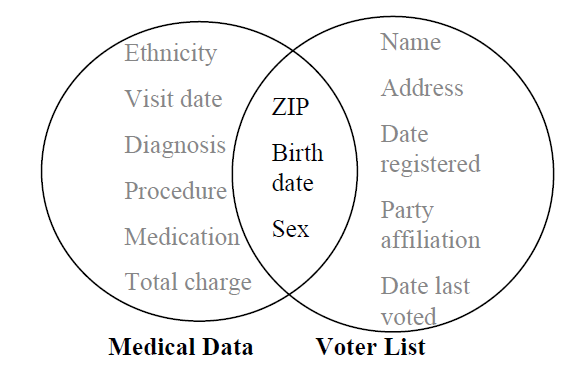
\includegraphics[width=0.6\textwidth]{linkingdata.png}
	\caption{Quasi-identifiers}%
	\label{quasiidentifier}
\end{figure}\\
The most important type of data worth mentioning is \textit{sensitive data}. This type of data is useful to researchers but they contain private information and should not be publicized or be accessible to strangers. Record owners do not want to be linked to these type of data. Next to data types there are 3 ground knowledge types: \textit{Background knowledge}, \textit{Instance-level background knowledge}, \textit{Demographic background knowledge}. \textit{Background knowledge} deals with the uncertainty of the amount of data access the attackers has. The developer has to consider that the attackers might have access to a table, since they know that in order to achieve k-anonymity tables are generalized. Furthermore, the attackers are aware of the domain attributes. Instance-level background knowledge, then, reveals that the adversary possesses comprehensive knowledge of the target’s specific details. For example, Alice (the adversary) knows that Bob does not suffer from a disease, because he has no symptoms. In this case, Alice can conclude of what actually Bob suffers from. Lastly, in the demographic background knowledge the adversary is informed about general facts, for example P (t[condition] = cancer| t[Age] 40). With these information the attackers can access and interference the records \cite{ldiversity}.\\\\
Considering \textit{K-Anonymity}, the main goal of making a k-anonymized table is to have at least (k-1) tuples of each identical tuple by taking the corresponding quasi-identifiers into account  \cite{sweeney2002k,li2006achieving}. For example, the k-anonymized version of \textit{Table  \ref{intro_example}} in the introduction section would be the following table:
\begin{table}[]
	\centering
	\caption{Basic example 2-anonymized}
	\label{intro_example_sol}
	\begin{tabular}{@{}llll@{}}
		\toprule
		SSN         & Age & Postcode & Problem         \\ \midrule
		* & 2*  & 456*     & stress \\
		* & 3*  & 456*     & stress          \\
		* & 4*  & 456*     & stomach cancer  \\
		* & 3*  & 456*     & obesity         \\
		* & 4*  & 456*     & stomach ulcers  \\
		* & 2*  & 456*     & stress          \\ \bottomrule
	\end{tabular}
\end{table}\\
The set of all tuples with the identical quasi-identifiers of a table are referred as equivalence class \cite{li2006achieving}.\\ \\
It is also important to note that there are two kinds of disclosure, \textit{ identity disclosure}, during which an individual is linked to a particular record. Due to this \textit{attribute disclosure} might occur, once new information about an individual are revealed. For example, Bob is linked to his record in \textit{Table \ref{intro_example_sol}}, because of some attack (see Section 3.2). The adversary discovers that he suffers from stress \cite{sweeney2002k}.\\\\
The last two terms concerning the basic concepts of k-anonymity are \textit{Global recoding/domain generalisation} and \textit{local recording}. The first refers to a very common generalization technique during which once an attribute value is generalized then all occurrences of that value are replaced by the generalized one  \cite{sweeney2002k,sweeney2002achieving,li2006achieving,incognito}. The later entails coding strategies, which work differently from the ones described above. \textit{Local recording} generalizes the attribute values in cells. Consequently, these types of strategies do not over generalize the table and the data distortion is significantly lower \cite{li2006achieving}. 
 
\section{Underlying Barriers}

In the following section, the paper will present the basic and most challenging barriers to the implementation of k-anonymity. The barriers, which can emerge during the implementation of k-anonymity, will be explained further. These are the so-called \textit{distortion of data}, or as mentioned in some papers \textit{data loss}. 
\subsection{Distortion of data as Barrier} \label{sec:Distortion of data as Barrier}

A basic underlying barrier of k-anonymity is the process of measuring whether an implementation has been successful or whether it leads to a satisfying result. This can be measured by a simple calculation. The \textit{modification rate} denotes the fraction of cells which are modified within the attribute set of the quasi-identifier \cite{li2006achieving}.

	
\begin{table}[]
	\centering
	\caption{a: original table, b: example for local recording, c: example for domain generalization }
	\label{table_distortion}
	\begin{tabular}{@{}lllllllllll@{}}
		\multicolumn{3}{c}{\textbf{a}} &           & \multicolumn{3}{c}{\textbf{b}} &  & \multicolumn{3}{c}{\textbf{c}} \\ \midrule
		Gender  & Birthday   & Problem & \textbf{} & Gender  & Birthday   & Problem &  & Gender  & Birthday  & Problem  \\ \midrule
		male    & 13.08.1962 & stress  &           & male    & 13.08.1962 & stress  &  & *       & 196*      & stress   \\
		male    & 28.10.1967 & obesity &           & male    & 28.10.1967 & obesity &  & *       & 196*      & obesity  \\
		male    & 20.01.1977 & stress  &           & *       & 197*       & stress  &  & *       & 197*      & stress   \\
		female  & 15.09.1973 & obesity &           & *       & 197*       & obesity &  & *       & 197*      & obesity  \\
		female  & 15.03.1985 & stress  &           & female  & 15.03.1985 & stress  &  & *       & 198*      & stress   \\
		female  & 28.05.1986 & obesity &           & female  & 28.05.1986 & obesity &  & *       & 198*      & obesity  \\ \bottomrule
	\end{tabular}
\end{table}

As can be observed in \textit{Table \ref{table_distortion}b}, the modification rate is  33,$\overline{33}$\% (4 out of 12 quasi-identifier are changed) but for \textit{Table \ref{table_distortion}c} the rate is 100\% (12 out of 12 quasi-identifier got changed). As it can be seen in this simple example, the modification rate calculation is an unsatisfying procedure. Due to this, Li, Wong, Fu and Pei introduced the \textbf{weighted hierarchical distance}. In order to calculate the weighted hierarchical distance of a cell which is generalized from level p to level q, the following formula is used\\
%%%%%%%%%%%%%%%%%%
%%%FORMEL%%%%%%%%%
%%%%%%%%%%%%%%%%%%
\scalebox{1.25}{$ WHD (p, q) = \frac{\sum_{j=q+1}^{p} \omega_{j,j-1}}{\sum_{j=2}^{h} \omega_{j,j-1}} $}\cite{li2006achieving}.\\
%%%%%%%%%%%%%%%%%%
%%%FORMEL%%%%%%%%%
%%%%%%%%%%%%%%%%%%
Let the hierarchy of birth date be \{D/M/Y, M/Y, Y, 10Y, C/T/G/P, *\}. Where D/M/Y  stands for day.month.year, 10Y a 10 years interval and C/T/G/R for Child/Teen/Grownup/Pensioner.
\\\\
Another example can be shown by having a uniformed weight $w_{j,j-1} = 1$ where $2\leq j \leq h$ \cite{li2006achieving}. By Using the aforementioned example Birthday is generalized from D/M/Y to 10Y, which corresponds into $WHD_{Birthday}(6,3) = \frac{3}{5} = 0,6$. 
The Gender generalization would be $WHD_{gender}(2,1) = \frac{1}{1} = 1$. In such, in order to generalize 5 cells of age from D/M/Y to 10Y, one has to do the same data distortion as when 3 cells of gender are generalized from Male/Female to *. This calculation presents a much better way to address the distortion of data than the modification rate. However, this does not take into account how close is the generalization to the root (which would be *).\\\\
A last example can be shown with height weight $w_{j,j-1} = 1 / (j-1)^{\beta}$ where 2 $\leq$ j $\leq$ h and $\beta = \R \geq$ 1 \cite{li2006achieving}:
$\beta$ can be chosen by the user. For example $\beta = 1$. For $WHD_{Birthday}(6,3) = \frac{0,\overline{33}+0,25+0,20}{1+0.5+0,\overline{33}+0,25+0,20} \sim 0,3431$. For $WHD_{gender}(2,1) = \frac{1}{1} = 1$. The distortion of almost 3 changed cell of birthday from D/M/Y to 10Y have the impact on the distortion as only one cell from Female/Male to * gets generalized.\\\\
Coming to a conclusion the researcher demands the information provided in the tables, as shown in these examples. Therefore, it is very important that the least possible information are lost during the anonymization process. In order to understand the importance of this aspect, consider another example. You a table with survivors from a disaster beyond all expectations. Researchers will try to discover the long-term effects of this disasters and whether the victims are more likely to live a long and happy life by measuring their distance from disaster’s location. If there is a mass generalization of by the location (ZIP), it might be useless or non-significant for researchers to work with this information.
%%%%%%
%% DONE %%%
%%%%%%%%%%%%%
\subsection{Attacks as Barrier}

Attacks can be considered as another barrier to k-anonymization implementations. If the implementation ignores the deficiencies which the attacks can make use of, k-anonymity has then no value. It is absolutely necessary that an attacker, under no circumstances, discovers information about the target while he/she is reading the published database. This should also be feasible even if the attacker has background knowledge of other sources   \cite{Dalenius1977}. Unfortunately, as shown by Dwork such safety parameters are impossible, because of the unfeasibility to predict what the attacker might know \cite{dwork2011differential}. Therefore, it is important and necessary that the implementation takes possible attacks into account and implements countermeasures. However, since attacks are not the main focus of this paper, a rather short introduction will be provided. 

\subsubsection{Homogeneity attack}

One type of an attack is the so-called \textit{Homogeneity Attack}. Let Alice be the adversary and let be Bob her target. They are neighbours and one day Bob is transported with an ambulance to the hospital. Let us assume that the hospital published the \textit{Table \ref{4ktable}}, where all current patients including their \textit{Nationality, Age, ZIP,} and \textit{Problem}, are listed, is already k-anonymized before its release. Alice knows that Bob is a 31 years old, American who lives in 02239 (ZIP Code). Thus, she can conclude that he is entry 3, 5,6, or 11.

Furthermore, all of these entries have the same Problem: Cancer. Alice can conclude that Bob suffers from cancer even if the table the table has already been k- anonymized  \cite{sweeney2002k,ldiversity}. To counteract such attacks diversity is needed \textbf{diversity}. One method which is worth mentioning, but will not be further discussed in this paper is the so-called l-diversity.  

% Please add the following required packages to your document preamble:
% \usepackage{booktabs}
\begin{table}[]
	\centering
	\caption{Homogeneity attack}
	\label{homogenityattack}
	\begin{tabular}{@{}llllllllll@{}}
		\cmidrule(lr){2-5} \cmidrule(l){7-10}
		& Nationality     & Age & ZIP   & Problem         &  & Nationality & Age      & ZIP   & Problem         \\ \cmidrule(lr){2-5} \cmidrule(l){7-10} 
		1  & American        & 42  & 02135 & Viral Infect    &  & *           & $\geq$40 & 021** & Viral Infect    \\
		2  & Japanese        & 41  & 02133 & Hearth disease  &  & *           & $\geq$40 & 021** & Hearth disease  \\
		3  & Germany         & 38  & 02238 & Hearth disease  &  & *           & 3*       & 0223* & Cancer          \\
		4  & Japanese        & 29  & 02139 & Fever           &  & *           & $\leq$30 & 021** & Fever           \\
		5  & Indina          & 37  & 02232 & Viral Infection &  & *           & 3*       & 0223* & Cancer          \\
		6  & Native-american & 34  & 02236 & Cancer          &  & *           & 3*       & 0223* & Cancer          \\
		7  & Russia          & 53  & 02138 & Viral Infection &  & *           & $\geq$40 & 021** & Viral Infection \\
		8  & China           & 23  & 02139 & Cancer          &  & *           & $\leq$30 & 021** & Cancer          \\
		9  & American        & 23  & 02141 & Short of breath &  & *           & $\leq$30 & 021** & Short of breath \\
		10 & Indian          & 46  & 02139 & Viral Infection &  & *           & $\geq$40 & 021** & Viral Infection \\
		11 & American        & 31  & 02239 & Vomiting        &  & *           & 3*       & 0223* & Cancer          \\
		12 & American        & 28  & 02130 & Viral Infection &  & *           & $\leq$30 & 021** & Viral Infection \\ \cmidrule(lr){2-5} \cmidrule(l){7-10} 
	\end{tabular}
\end{table}

Another type of an attack is the \textit{Background Knowledge Attack}. This type of an attack uses demographic background knowledge, which is stored in the ground information of an adversary. Let us assume that Alice has a colleague, who enters also to the same hospital. This colleague is a 32 years old, Japanese and lives in 93607 (ZIP). Everyone with the same quasi-identifiers, i.e. Age = 3* and ZIP = 936**) have cancer or a heart disease. However, she knows that Japanese have a very low risk of a heart disease and, thus, she concludes that her college has cancer \cite{ldiversity}.
\begin{table}[]
	\centering
	\caption{Background Knowledge Attack}
	\label{tablebackground}
	\begin{tabular}{@{}llllllll@{}}
		\cmidrule(r){1-4} \cmidrule(l){6-8}
		& ZIP Code & Age & Disease        &  & ZIP Code & Age      & Disease        \\ \cmidrule(r){1-4} \cmidrule(l){6-8} 
		1 & 93677    & 29  & Liver Disease   &  & 936**    & $\leq$30 & Liver Disease   \\
		2 & 93602    & 22  & Liver Disease   &  & 936**    & $\leq$30 & Liver Disease   \\
		3 & 93909    & 52  & Cancer         &  & 9390*    & $\geq$40 & Cancer         \\
		4 & 93906    & 47  & Flu            &  & 9390*    & $\geq$40 & Flu            \\
		5 & 93673    & 36  & Hearth Disease &  & 936**    & 3*       & Hearth Disease \\
		6 & 93607    & 32  & Cancer         &  & 936**    & 3*       & Cancer         \\ \cmidrule(r){1-4} \cmidrule(l){6-8} 
	\end{tabular}
\end{table}

The last type of attack that will be shown in this table is the Unsorted Matching Attack against k-anonymity. This type of attack is based on the very common strategy to release two tables separately. For example, let us assume a two column weight \textit{Table \ref{MatchingAttack}a}. This table can then be separated into two tables (6b, 6c). \textit{Table \ref{MatchingAttack}b} will contain \textit{Age} completely generalized but ZIP ungeneralized, and \textit{Table \ref{MatchingAttack}c} will have \textit{Age} ungeneralized but ZIP is generalized. The adversary can simply merge both tables and obtain \textit{Table \ref{MatchingAttack}a}, and have access to sensitive information. This weakness can be solved through random sorting \cite{meyerson2004complexity}.

\begin{table}[]
	\centering
	\caption{Unsorted Matching Attack example}
	\label{MatchingAttack}
	\begin{tabular}{@{}cccccccc@{}}
		\multicolumn{2}{c}{\textbf{a}} & \multicolumn{1}{l}{} & \multicolumn{2}{c}{\textbf{b}} & \multicolumn{1}{l}{} & \multicolumn{2}{c}{\textbf{c}} \\ \cline{1-2} \cline{4-5} \cline{7-8} 
		Age           & ZIP            &                      & Age           & ZIP            &                      & Age           & ZIP            \\ \cline{1-2} \cline{4-5} \cline{7-8} 
		42            & 91058          &                      & *             & 91058          &                      & 42            & 91050          \\
		44            & 91058          &                      & *             & 91058          &                      & 44            & 91050          \\
		50            & 27785          &                      & *             & 27785          &                      & 50            & 27780          \\
		52            & 27785          &                      & *             & 27785          &                      & 52            & 27780          \\
		20            & 32105          &                      & *             & 32105          &                      & 20            & 32100          \\
		21            & 32105          &                      & *             & 32105          &                      & 21            & 32100          \\
		31            & 67676          &                      & *             & 67676          &                      & 31            & 67670          \\
		32            & 67676          &                      & *             & 67676          &                      & 32            & 67670          \\ \cline{1-2} \cline{4-5} \cline{7-8} 
	\end{tabular}
\end{table}

Drawing a conclusion from the possible attacks on \textit{k-anonymity}, it should be clear that before the implementation of \textit{k-anonymity} the application has to be tested for such attacks it should also be secured against any other possible attacks.

\subsection{NP Hard}
Meyerson and Williams analyze the production of an optimal K-anonymity solution in their complexity and found out that it is an NP-Hard Problem. Which means that the problem is at least NP-Complete but maybe harder. The Algorithm which should produce optimal K-anonymity will maybe not find a solution. Concerning a real world application, this means that the production of a k-anonymity solution with the least possible information loss is not feasible. However they show an approximation algorithm for k-anonymizing, which will take polynomial time and will use suppression the most O(k log k)  \cite{sweeney2002k}. The problem with suppression is the high information loss it produces. So someone had to choose between time complexity and information loss as a barrier for the implemenation of k-anonymity \cite{el2009globally}. 



\section{Algorithm}
This section will show some algorithms which goals is to archive \textit{k-anonymity} through generalization. 

\subsection{The KACA Algorithm}
The idea behind this algorithm idea is to achieve \textit{k-anonymity} by clustering attribute hierarchical structures. The algorithm chooses a random \textit{equivalent class}, which is smaller than k. The next step is to form a lager \textit{equivalent class} by merging the chosen one with the closest \textit{equivalent class}. This is resulting in a larger combined \textit{equivalent class}. Through repeating this process the end result is that each \textit{equivalent class} consists of at least k-tuples \cite{li2006achieving}.\\
\begin{algorithm}[H]
	\caption{K-Anonymization by Clustering in Attribute hierarchies (KACA) \cite{li2006achieving}}
	form equivalence classes from the data set\\
	\While{there exists an equivalence class of size $<$ k}{
	randomly choose an equivalence class $C$ of size $k$ k\\
	evaluate the pairwise distance of $C$ and all other equivalence classes\\
	find the equivalence class $C'$ with the smallest distance to $C$\\
	generalise the equivalence classes $C$ and $C'$
	}	
\end{algorithm}
This algorithm has a runtime of $O(nlogn + |E|^{2})$. Li, Wong, Fu, and Pei have shown that their \textit{KACA-Algorithm} is resulting in a 5.57 times smaller amount of distortion as the well known \textit{Incognito Algorithm}. The reason is lying in the technique which \textit{Incognito} is using. Its a global recoding algorithm, which is resulting in a over-generalized table \cite{li2006achieving}.


\subsection{The OLA Algorithm }

The OLA Algortihm was original produced for the field of health data anonymization. Also he wants to prodcue optimal k-anonymity. That means producing the usual definition of k-anonymity with the differents to produce less information loss as possible. In chapter \ref{sec:Distortion of data as Barrier} was shown one possibilty of measuring the information loss. 
The Algortihm can use 3 different Kind of Information loss metrices which result in different anonymization result. Information loss can result in loss of statistical power, inaccurate analysis result and inefficient use of data.  The alogrithem works with supression and generalization of the data. Supression can result in drastical information loss due to the fact that a hole attribute gets raced.  Generalization will performed on all potential Quasi identifiers. An example for generalization can be found in figure \ref{Generalization}.For different kind of data there a different kind of genralization techniks. So for strings the rightmost char can be deleted. For numerical data we can produce intervals which will include the generalicate attribute. For date we can reduce the specifikation from days to months till years. Generalization includes Supression. The hightes attribute on each generalication lattice is the supressed version of the attribute in includes no information at all \cite{el2009globally}. The most time consuming operation is finding the all the K-anonymous notes and comparing them to each other with respect to information loss. In order to achieve a better performance at the Programm step 1) the OLA algorithm uses Predictive Tagging which enhances the process.  This Tagging take advantage of the structure of the generalization Lattice. A lattice is shown in Figure \ref{lattice}. That every k-anonymous note in the same generalization lattice on hight n. All notes above n and in the same generalization strategy are also k-anonymous. So the algorithm only has to find the first k-anonymous note in the strategy and tag all above this node as k-anonymous.

\begin{figure}
	\centering
	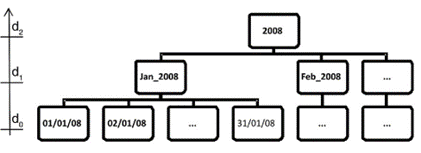
\includegraphics[width=0.6\textwidth]{general1.png}
	\caption{Generalization}%
	\label{Generalization}
\end{figure}

\begin{figure}
	\centering
	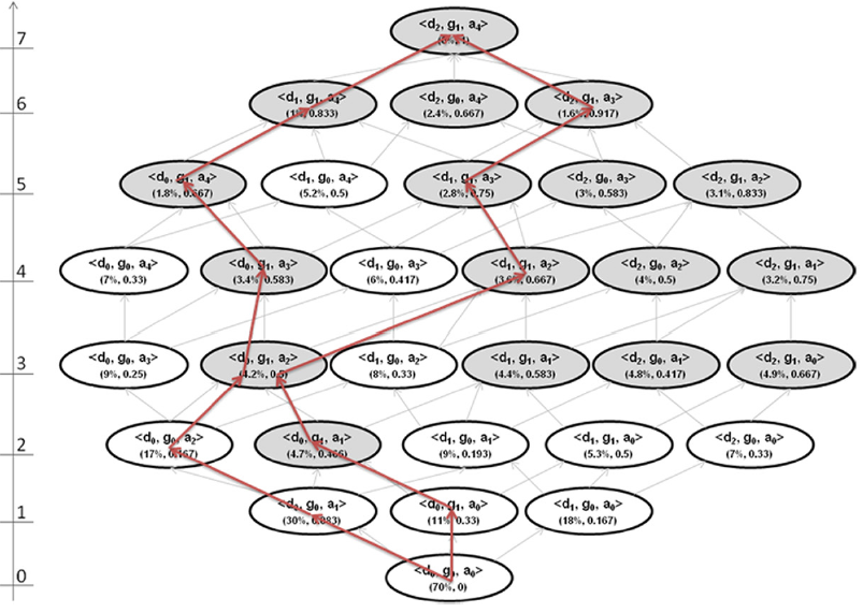
\includegraphics[width=0.6\textwidth]{lattice.png}
	\caption{Generalization Lattice}%
	\label{lattice}
\end{figure}


\begin{algorithm}[H]
\caption{The OLA Algorithm works in 3 Steps:}
\While{not all generalization strategies are compared}
{
 For every generalization, strategy builds a binary search to find all k-anonymous nodes in the different strategies\\
For every generalization strategy that includes k-anonymous nodes save the one with the least Information loss in the hole generalization strategy, this is referred to a local option k-anonymous solution\\
Compare the local optimum solutions to respect of the information loss. The one with the lowest Information loss of all local optimum solutions is the global optimum solution\\
\Return{global optimal solution}
}
\end{algorithm}

The Information loss can be measured with three possible matrices. The hight of each generalized attribute can be taken as a measure. As an example in figure \ref{Generalization} if we generalize on Level d1. We would have an information loss of one. The problem with that kind of measurement is that it doesn´t take into account the hight of the hole generalization tree. If we would generalize the gender of a person than we only have one possibility. The specific gender or no information at all. With the first measurement, we also would measure an information loss of one. To get rid of that problem someone can use the Prec measurement. It takes into account the total possible hight of the generalization tree. It can be measured with this formula
{\text{Number of levels generalized}}{/\text{Number of possible generalization levels} = Information loss. The last possibility is Discernability Metric(DM). It gives a penalty to each record that is indistinguishable from other records. So if we generalize less there will be less penalty. Another barrier for a general practice of k-anonymity algorithm is that it measures the information loss in their data set. After all, the anonymized dataset will be used in datamining applications and there is no possibility to measure the information loss regarding the goal of the data mining. So for the OLA algorithm, there is a possibility to not find a solution at all due to the fact it´s and NP-Hard problem to find an optimal k-anonymity solution\cite{el2009globally}.



\subsection{Cloaking Algorithm}
Moving object data creates new challenges to a traditional database, data mining, and privacy-preserving technologies due to its unique characteristics. It is time-dependent, location-dependent, and is generated in large volumes of high-dimensional stream data. The following algorithm provides an example of privacy production. The Cloaking Algorithm tries to produce anonymity on location-based data for users of Location Bases Services(LBS). The Cloaking Algorithm is installed on a location protection broker on a trusted server and anonymize messages which will afterward send to the LBS. K-anonymity prevents such a privacy breach by ensuring that each individual record can only be released if there is at least k − 1 other (distinct) individuals whose associated records are indistinguishable from the former in terms of their quasi-identifier values. There a two possible attacks which can obtain  the identity of a sender of a message. In  Restricted Space Identification, the attacker (A) observes that message (M) is sent from location(L).He then detects the background knowledge that L belongs to someone specific. For example, if Mr. Bob the owner of a flat sends a message and the attacker observes this message. He can re-link the identity of Bob. Another Attack is  Observation Identification. If A has observed the current location L of subject S and finds a message M from L then A learns that S has sent M.  To prevent this leaking of information the cloaking algorithm works with Spatial Cloaking and Temporal Cloaking. Spatial Cloakings goal is to increase the location from where M is sended in such a way that there are more messages in this area. So that there is not only one message at a time in one area. Temporal Cloaking extends the sending time until more messages are in one area. With these both technics the algorithm tries to produce k-anonymity for m different messages. With the possibilty of delaying a message with the Temporal Cloaking until enough messages are in one location wil harm the usability of the LBSs. In der Paper Gedik and Liu shown is is possible to implement on a real world example but it will lack on the utility of the LBS because of the delaying  messages \cite{gedik2004customizable}.



\section{High-Dimensional Transaction Data}

Transaction dada is typical high-dimensional. Shopping sites like Amazon.com got millions of catalog items which all could be a potential QID and therefor must be k-anonymitats before publishing this kind of data \cite{wang2010privacy}. Aggarwal shown in his paper "On k-Anonymity and the Curse of Dimensionality" that this task is impossible to archive. They work with a clustering K-anonymity algorithm like The KACA Algorithm and try to archive 2-anonymity on a 3108 dataset. He shows with the increase of the dimension of the dataset and the goal to archive k-anonymity the information loss increase rapidly till a point of not practical for applications like data mining tools.  The reason for that is the curse of high dimensionality which doesn't allow the clustering of points because of too much space between them. Xu introduced a method to get at least a bit of practical usage. He proclaimed that an attack knows at least n-different transactions of a victim and concludes that some information can get \cite{xu2008publishing}. So he said that that the backgroundknowlwege of an attacker in bounded \cite{aggarwal2005k}. 

%\section{Releated techniques}
\section{Summary}
Like we saw in section OLA algorithm there are possibilities of choosing between different information loss metrics which all compute different values to the same k-anonymous node. So the implementer has to choose which one fits the most in his data. Different Metrics have pros and contras and have to be compared. Another problem with Information loss is that you can measure the information loss on your dataset but what would be more is interesting the information loss compared to upcoming data mining tool or machine learning application. The information loss metrics can´t know which information is important for the upcoming data mining step.suppression can also harm the quality of the data and should be chosen wisely.The production of k-anonymity is NP-Hard which results in a difficult implementation in real-time applications like the Cloaking - Algorithm had shown. This Complexity can result in problems of finding an optimal solution in real-world data sets and can make a practical implementation difficult. High Dimensional Data like transaction data with more than thousand of attributes are in practice not capable to produce k-anonymity for all attributes. The reason for that is the so called Curse of High Dimensionality which produces a metric space which is too large to produce k-anonymity solutions for all attributes. A  Possibility is so called, bounded background knowledge that some attributes can´t be used as a quasi-identifier because the effort of getting background knowledge which can be linked to the attributes is estimated too high. Like shown i chapter {Attacks as Barrier} attacks against k-anonymity are a threat for the anonymity of the user and can result in identity disclosure.There solutions regarding these kind of attacks we proposed in this paper. L-Diversity and T-Closeness will help against them. The cloaking algorithm shoves a good example of the connection between anonymity and usability. The anonymization of the data reduces the usability of location-based services. Which comes from the construction of the Spatial cloaking and Temporal cloaking boxes to have enough messages to constrain them and let the be k-anonymous. The Software gives the option that a user of the client can decide how much usability he wants to sacrifice to get anonymity. So the user is at least under the control of how much utility he wants to give up. 

\newpage
\bibliography{literature}
\bibliographystyle{splncs03}

\end{document}


